\documentclass{article}

% DO CHAPTERS 1 3 4 AND 5

\usepackage[margin=0.75in]{geometry}
\usepackage{hyperref}
\usepackage{listings}
\usepackage{fontspec}
\usepackage{graphicx}

\graphicspath{ {./images/} }

\setmonofont{Consolas}

\setlength{\parindent}{0pt}

\hypersetup{
    colorlinks,
    linkcolor=blue,
}

\lstset{basicstyle=\ttfamily}

\title{Applied Recommender Systems — A Report}
\author{Lakshit Verma}

\begin{document}

\maketitle
\tableofcontents
\newpage

\section{Introduction}

This report is a short summary of the book \textbf{Applied Recommender Systems with Python}. It covers chapters 1, 3, 4 and 5 of the text respectively. In the initial chapter, we get a brief introduction to the world of recommendation systems and their types. In the subsequent chapters, we get a deeper dive into three methods of recommendation— Content-Based, Collaborative Filtering, and the methods used to achieve and improve on Collaborative Filtering.

\section{Introduction to Recommendation Systems}

recommendation systems are typically built for one purpose— to maximize revenue by enhancing the user's experience and maximize their time spent on the site.
To build a recommendation system, the most crucial element is user feedback. This comes in two forms, \textbf{explicit} and \textbf{implicit}.

\begin{itemize}

    \item{\textbf{Explicit Feedback:} It is feedback the user knowingly and explicitly puts on a product. Examples of this include likes, dislikes, star ratings, and reviews.}
    \item{\textbf{Implicit Feedback:} This is the feedback that is generated unconsciously, through the revealed preferences of the user. These can include links clicked on, pages visited, video watch time, etc.}

\end{itemize}

\subsection{Types of recommendation engines}

There are several methods of creating a recommendation engine. The ones given in the text are as follows:

\begin{enumerate}
	\item{\textbf{Market basket analysis (association rule mining)}}
	\item{\textbf{Content-based filtering}}
	\item{\textbf{Collaborative-based filtering}}
	\item{\textbf{Hybrid systems}}
	\item{\textbf{ML clustering}}
	\item{\textbf{ML classification}}
	\item{\textbf{Deep learning and NLP}}
\end{enumerate}

\subsubsection{Market basket analysis}

This is method most often used by retailers to predict the popularity of a given item. It works through identifying pairs of items that are often put together.

\medskip

A few important terms are used in context of this system, and one of them is \textbf{Association rule}. Their purpose is to identify and symbolize strong relationships between items. They are written in the form \texttt{\{antecedent→consequent\}}. For example, take \texttt{\{bread→jam\}}, which means in plain English \textbf{``There is a strong relationship between customers who bought bread and jam in the same purchase''}.

\medskip

\textbf{Support} is the relative frequency of an association rule displaying. \textbf{Confidence} measures the reliability of the rule, where a confidence of 0.5 indicates the items in question were purchased together 50\% of the time. Finally, \textbf{Lift} is a measure of the ratio of the expected support vs. the support if two rules are independent. A lift value close to one means the rules are independent, and lift values over 1 indicate more and more correlation between the two rules.

\subsubsection{Content-Based Filtering}

Content-based filtering method is a recommendation algorithm that suggests items similar to the ones other users have previously selected or shown interest in.

\medskip

Take the example of Netflix. The popular streaming site saves all user viewing information in a vector-based format, known as the \textbf{profile vector}, which contains information on past viewings, liked and disliked shows, most frequently watched genres, and so on. Then there is another vector that stores all the information regarding the titles (movies and shows) available on the platform, known as the \textbf{item vector}. It stores information like the title, actors, genre, language, length, crew info, synopsis, etc.

\medskip

The content-based filtering algorithm uses the concept of cosine similarity. In it, you find the cosine of the angle between two vectors — the profile and item vectors in this case. Suppose \( A \) is the profile vector and \( B \) is the item vector, then the (cosine) similarity between them is calculated as follows:

$$ sim(A, B) = \cos{\theta} = \frac{A \cdot B}{\|A\| \|B\|} $$

This outcome always ranges between -1 and 1, and is calculated for multiple item vectors, keeping the profile vector constant. They are then ranked in descending order of similarity, and have one of two following approaches applied for recommendations:

\begin{itemize}
    \item{\textbf{Top-N approach:} The top N movies are recommended, where N limits the number of titles recommended.}
    \item{\textbf{Rating scale approach} A limit on the similarity value is set, and all the titles satisfying that threshold are recommended.}
\end{itemize}

Other methods such as \textbf{Euclidean Distance} ($ \sqrt{(x_1 - y_1) ^ 2 + \cdots + (x_N - y_N) ^ 2} $) and \textbf{Pearson’s correlation} are also utilized in select cases.

\medskip

The critical flaw of such a system is the fact that all suggestions emerging from this end up falling into the same sort of product ``category'', making it feel formless and repetitive.

\subsubsection{Collaborative-Based Filtering}

In this, a user-user similarity is considered along with item similarities, to address the issues with simple Content-Based filtering.

\medskip

The process of finding similarities is much the same as that of Content-Based filtering, but the engine then recommends titles that the user has not watched but other users with the same interests have. There are two kinds of Collaborative-Based filtering algorithms.

\begin{itemize}
    \item{\textbf{User-user collaborative filtering:} Here, you find user-user correlations and offer recommendations based on what similar users chose before. Despite its effectiveness, it is highly compute-intensive and its use in large-scale databases is therefore discouraged.}
    \item{\textbf{Item-item collaborative filtering:} This involves finding similarities in item-item pairs instead of user-user pairs. This is far less computationally demanding, at the cost of less accurate results.}
\end{itemize}

\subsubsection{Hybrid Systems}

A hybrid system offers the best of both worlds— combining both content-based and collaborative-based systems, drawing power from another when one fails to produce desirable results. They can be implemented in the following ways:

\begin{itemize}
    \item{Generating recommendations separately by using content- and collaborative-based systems and merging them subsequently.}
    \item{Adding features of the collaborative method to a content-based recommender engine.}
    \item{Adding features of the content method to a collaborative-based recommender engine.}
\end{itemize}

Studies consistently show that hybrid recommender engines generally perform better, faster and provide more reliable recommendations.

\subsubsection{ML clustering}

Applying the novel field of Machine Learning to the recommendation systems seems like the logical next step. ML methods are of two types: supervised and unsupervised. Clustering is the unsupervised method, meaning it finds patterns in data sans any human intervention in labelling the data. It is the process of grouping objects into clusters, and generally an object belonging to a cluster is more similar to the objects inside the cluser than the objects outside of it.

\medskip

Clustering based methods are usually implemented when there is little user data to go by. If a user is found to be similiar to a cluster of users, the user is added to that cluster. Users inside the cluster all share specific tastes, and recommendations are provided according to that.

\medskip

Some popularly used clustering algorithms are:

\begin{itemize}
	\item{\textbf{K-means clustering}}
	\item{\textbf{Fuzzy mapping}}
	\item{\textbf{Self-organizing maps (SOM)}}
	\item{\textbf{Hybrids of two or more techniques}}
\end{itemize}

\subsubsection{ML classification}

In a classification based system, the algorithm uses features of both the items and users to predict a user's affinity towards a given product. One application of this is the buyer propensity model.

\medskip

Some flaws of classification-based systems are:

\begin{itemize}
    \item{Collection of data is tedious.}
    \item{Its classification is challenging, and again, time-consuming.}
    \item{Training the models to function in real time is difficult.}
\end{itemize}

\subsubsection{Deep Learning}

Deep Learning and Deep Neural Networks (DNNs) are a more powerful form of Machine Learning. They work especially well on unstructured data such as text, images, and video.

A few DL-based systems are:

\begin{itemize}
    \item{\textbf{Restricted Boltzmann}}
    \item{\textbf{Autoencoder based}}
    \item{\textbf{Neural Attention based}}
\end{itemize}

\subsection{Applications}

Here, we look at real examples of the construction of recommendation systems using Python and sci-py.

\subsubsection{Popularity}

This is the simplest form of recommendation— to sort products based on a measure of popularity (views, downloads, likes, etc.)

\medskip

We import the required libraries and data first.

\begin{lstlisting}
import pandas as pd
import numpy as np
import seaborn as sns
import matplotlib.pyplot as plt

df = pd.read_csv('data.csv',encoding= 'unicode_escape')
\end{lstlisting}

Cleaning up the data by dropping NULLs and values with no description, we finally sort the most popular items.

\begin{lstlisting}
global_popularity=df_new.pivot_table(index=["StockCode","Description"],
values="Quantity", aggfunc="sum").sort_values(by="Quantity", ascending=False)
print("10 most popular items globally....")
global_popularity.head(10)
\end{lstlisting}

To calculate the most popular items by country, we use the following code:

\begin{lstlisting}
# Popular items by country
countrywise=df_new.pivot_table(index=["Country","StockCode","Description"],
values="Quantity", aggfunc="sum").reset_index()

# Vizualize top 10 most popular items in UK
sns.barplot(y="Description", x="Quantity",
    data=countrywise[countrywise["Country"] == "United Kingdom"]
        .sort_values(by="Quantity", ascending=False).head(10))
plt.title("Top 10 Most Popular Items in UK", fontsize=14)
plt.ylabel("Item")
\end{lstlisting}

\subsubsection{Buy Again}

This is another simple system that sorts items by number of repeated instances, and recommends the ones at the top.

\begin{lstlisting}
from collections import Counter

def buy_again(customerid):
# Fetching the items bought by the customer for provided customer id
items_bought = df_new[df_new["CustomerID"] == customerid].Description

# Count and sort the repeated purchases
bought_again = Counter(items_bought)

# Convert counter to list for printing recommendations
buy_again_list = list(bought_again)

# Printing the recommendations
print("Items you would like to buy again :")

return(buy_again_list)
\end{lstlisting}

Using the function on a specific user, say 1252 (function call \texttt{buy\_again(1252)}), we will recieve a list of the most likely items the user is to buy, based on their previous purchase history.

\section{Content-Based Recommender Systems}

Content-Based filtering systems recommend products based on their similarity to products already having piqued the user's interest, indicated through buying, liking, reviewing, etc.

\medskip

The steps to build a Content-Based recommendation system are:

\begin{enumerate}
    \item{\textbf{Data collection}}
    \item{\textbf{Data preprocessing}}
    \item{\textbf{Conversion of text to features}}
    \item{\textbf{Performing similarity measures}}
    \item{\textbf{Recommendation of products}}
\end{enumerate}

\subsection{Data Collection}

To begin training, a bit of boilerplate code and imports are needed

\begin{lstlisting}
from sklearn.feature_extraction.text import CountVectorizer
from sklearn.metrics.pairwise import cosine_similarity,
    manhattan_distances,
    euclidean_distances
from sklearn.feature_extraction.text import TfidfVectorizer

from gensim import models

import pandas as pd
import numpy as np
import matplotlib.pyplot as plt
import matplotlib.style

from gensim.models import FastText as ft
from IPython.display import Image

import re
import os
\end{lstlisting}

A few models have already been trained on this, which we'll use. They are listed below

\begin{itemize}
    \item{\textbf{Word2vec:} \url{https://drive.google.com/uc?id=0B7XkCwpI5KDYNlNUTTlSS21pQmM}}
    \item{\textbf{GloVe:} \url{https://nlp.stanford.edu/data/glove.6B.zip}}
    \item{\textbf{fastText:} \url{https://dl.fbaipublicfiles.com/fasttext/vectors-crawl/cc.en.300.bin.gz}}
\end{itemize}

We then import the data: \texttt{Content\_df = pd.read\_csv("Rec\_sys\_content.csv")}

The columns of the table are as follows:

\begin{lstlisting}
>>> Content_df.info()
<class 'pandas.core.frame.DataFrame'>
RangeIndex: 3958 entries, 0 to 3957
Data columns (total 6 columns):
 #   Column        Non-Null Count  Dtype
---  ------        --------------  -----
 0   StockCode     3958 non-null   object
 1   Product Name  3958 non-null   object
 2   Description   3958 non-null   object
 3   Category      3856 non-null   object
 4   Brand         3818 non-null   object
 5   Unit Price    3943 non-null   float64
\end{lstlisting}

Now we load the pre-trained models.

\begin{lstlisting}
word2vecModel = models.KeyedVectors.load_word2vec_format(
    'GoogleNews-vectors-negative300.bin.gz', binary=True
)

fasttext_model=ft.load_fasttext_format("cc.en.300.bin.gz")

glove_df = pd.read_csv('glove.6B.300d.txt', sep=" ", quoting=3, header=None, index_col=0)

glove_model = {key: value.values for key, value in glove_df.T.items()}
\end{lstlisting}

\medskip

We now need to preprocess the text before turning it into features. This has the following steps.

\begin{enumerate}
    \item{Remove duplicates}
    \item{Convert the string to lowercase}
    \item{Remove special characters}
\end{enumerate}

\subsection{Features}

Now, we convert the text into Features. This can be done through several methods.

\begin{itemize}
    \item{\textbf{One-hot Encoding (OHE):} This is a simple technique. It converts all the tokens in the list of unique words to columns. Then, on every input, it turns the column of the word to the value 1 if present, and 0 if not.}
    \item{\textbf{CountVectorizer:} This is the same as OHE, except it keeps track of the number of times a word occurs and stores that in the column.}
    \item{\textbf{TF-IDF:} It addresses the problems in CountVectorizer by keeping track of two values, TF (term frequency) — the number of times a token appears in a corpus doc divided by the number of tokens, and IDF (inverse document frequency), which is the log of the total number of such corpus docs. It helps provide more weightage to rare words in the corpus. Multiplying this gives us a value referred to as the TF-IDF vector of the corpus.}
    \item{\textbf{Word Embeddings:} TF-IDF doesn't help in capturing the context of a sentence. To fix this, we use word embeddings. They are of several types, which are listed below.}
    \begin{itemize}
			\item{\textbf{Word2vec}}
			\item{\textbf{GloVe}}
			\item{\textbf{fastText}}
			\item{\textbf{Elmo}}
			\item{\textbf{SentenceBERT}}
			\item{\textbf{GPT}}
    \end{itemize}
\end{itemize}

\subsection{Similarity Features}

After converting text to features, we then employ a number of techniques to find similarity between words. They are of typically of three types.

\begin{itemize}
    \item{\textbf{Euclidean Distance:} It is calculated by taking the sum of the squares of two vectors and finding their square root.}
    \item{\textbf{Cosine Similarity:} This is the cosine of the angles between two vectors. It is essentially their dot product divided by the product of their magnitudes.}
    \item{\textbf{Manhattan Distance:} It's the sum of the absolute differences between two vectors.}
\end{itemize}

\subsection{Implementation}

We use CountVectorizer here as an example conversion model.

\begin{lstlisting}
# Comparing similarity to get the top matches using count Vec
def get_recommendation_cv(product_id, df, similarity, n=10):
    row = df.loc[df['Product Name'] == product_id]
    index = list(row.index)[0]
    description = row['desc_lowered'].loc[index]
    #Create vector using Count Vectorizer
    count_vector = cnt_vec.fit_transform(desc_list)
    if similarity == "cosine":
        sim_matrix = cosine_similarity(count_vector)
        products = find_similarity(sim_matrix , index)
    elif similarity == "manhattan":
        sim_matrix = manhattan_distances(count_vector)
        products = find_manhattan_distance(sim_matrix , index)
    else:
        sim_matrix = euclidean_distances(count_vector)
        products = find_euclidean_distances(sim_matrix , index)
    return products
\end{lstlisting}

The input for this is as follows

\begin{itemize}
    \item{\textbf{product\_id:} The product name for which we are finding similar reccomendations for.}
    \item{\textbf{df:} The preprocessed data.}
    \item{\textbf{similarity:} The similarity method to be run.}
    \item{\textbf{n:} Number of reccomendations.}
\end{itemize}

Now, lets take a word embedding of choice, say TF-IDF.

\begin{lstlisting}
# Comparing similarity to get the top matches using TF-IDF
def get_recommendation_tfidf(product_id, df, similarity, n=10):
    row = df.loc[df['Product Name'] == product_id]
    index = list(row.index)[0]
    description = row['desc_lowered'].loc[index]
    #Create vector using tfidf
    tfidf_matrix = tfidf_vec.fit_transform(desc_list)
    if similarity == "cosine":
        sim_matrix = cosine_similarity(tfidf_matrix)
        products = find_similarity(sim_matrix , index)
    elif similarity == "manhattan":
        sim_matrix = manhattan_distances(tfidf_matrix)
        products = find_manhattan_distance(sim_matrix , index)
    else:
        sim_matrix = euclidean_distances(tfidf_matrix)
        products = find_euclidean_distances(sim_matrix , index)
    return products
\end{lstlisting}

The output it gives us for \texttt{product\_id = 'Vickerman 14" Finial Drop Christmas Ornaments, Pack of 2'} is as follows:

\begin{center}
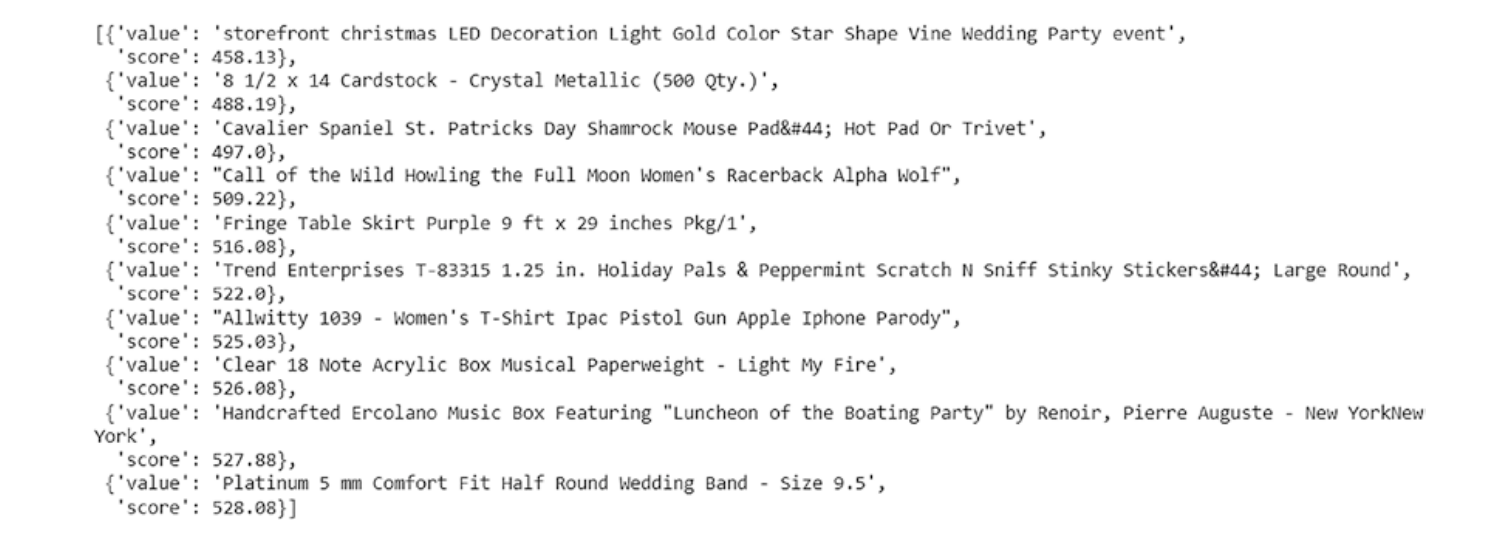
\includegraphics[scale=0.35]{01.png}
\end{center}

\section{Collaborative Filtering}
\section{C Filtering using Matrix Factorizing, Singular Value Decomposition, and Co-Clustering}

\end{document}
